%%%%%%%%%%%%%%%%%%%%%%%%%%%%%%%%%%%%%%%%%%%%%%%%%%%%%%%%%%%%%%%%%%%%%%%%%%%%%%%%
%2345678901234567890123456789012345678901234567890123456789012345678901234567890
%        1         2         3         4         5         6         7         8

%\documentclass[letterpaper, 10 pt, conference]{ieeeconf}  % Comment this line out
                                                          % if you need a4paper
\documentclass[a4paper, 10pt, conference]{ieeeconf}      % Use this line for a4
                                                          % paper

\IEEEoverridecommandlockouts                              % This command is only
                                                          % needed if you want to
                                                          % use the \thanks command
\overrideIEEEmargins
% See the \addtolength command later in the file to balance the column lengths
% on the last page of the document



% The following packages can be found on http:\\www.ctan.org
%\usepackage{graphics} % for pdf, bitmapped graphics files
%\usepackage{epsfig} % for postscript graphics files
%\usepackage{mathptmx} % assumes new font selection scheme installed
%\usepackage{times} % assumes new font selection scheme installed
%\usepackage{amsmath} % assumes amsmath package installed
%\usepackage{amssymb}  % assumes amsmath package installed
\usepackage[inline]{enumitem}
\usepackage[]{algorithm2e} %for pseudocode
\usepackage{graphicx}	% For figure environment
\usepackage[toc,page]{appendix}


\title{\LARGE \bf
CS433 Machine Learning Project 1
}

\author{Francesco Bardi, Samuel Edler von Baussnern, Zeya Yin % stops a space
}


\begin{document}



\maketitle
\thispagestyle{empty}
\pagestyle{empty}


%%%%%%%%%%%%%%%%%%%%%%%%%%%%%%%%%%%%%%%%%%%%%%%%%%%%%%%%%%%%%%%%%%%%%%%%%%%%%%%%



%%%%%%%%%%%%%%%%%%%%%%%%%%%%%%%%%%%%%%%%%%%%%%%%%%%%%%%%%%%%%%%%%%%%%%%%%%%%%%%%
\section{INTRODUCTION}

This project's goal was to tackle the Kaggle Higgs Boson challenge as part of
the \textit{CS433 Machine Learning} course at \textit{EPFL}. This challenge is 
to distinguish between two events: one being noise the other being the
detection of a Higgs Boson. We tried multiple linear models (constrained
by the exercise), feature selection methods and more complex multi-model design
methods.  The highest score on Kaggle's hidden data set was over 0.82.

\section{Data Analysis}

The data set consist of 30 features and 250000 observations, all but one
variables are numeric the other one being categorical, referred to as jet. A binary class label is
also given. Roughly half of the features are based on the other half and show a
high correlation. The variables show different value-ranges, standardisation is thus highly required.
The data set is unbalanced, with a 65.7\% being noise. This ratio varies for each subset defined by its jet.

\section{Outline}

Our simple model consists of two steps: 

\begin{enumerate*}[label={\alph*)}]
\item Pre-Processing \& Feature Engineering
\item Fitting the model
\end{enumerate*}

We outline these steps in more detail below.\\

Our final model however consists of multiple simple-models, each with it's own
set of parameters and weights. It wraps the above mentioned two steps around a subset selection based on the categorical value \texttt{PRE\_jet\_num}.

\section{Pre-Processing \& Feature Engineering}

This steps consists of both basic data handling as well as feature engineering.
When ever applicable the transformation is \textit{learned} using the
\textit{training set} and the same transformation is then applied on the
\textit{test} and \textit{prediction set}, we denote this with the term \textit{[...] is stored}. As some of these steps are
intertwined we present them in the order of application.

\subsection{Removal of redundant features}

Redundant features, identified by the absolute value of the pair-wise
correlation which exceed a certain threshold, are being removed. The list of
these features is stored.

\subsection{Removal of features with too many undefined values}

Features where the amount of undefined values is too large are removed. The
list of these features is stored.

\subsection{Dummy encoding of categorical values}

We only identified one categorical feature \texttt{PRE\_jet\_num}. A dummy
encoding was added to the feature matrix. The old column was removed. This applies only to the single-model case (see \ref{subsection:multimodel}).

\subsection{Feature Expansion}

In order to overcome the linearity of the given classifiers we add multiple
transformations of the base features to the feature matrix:\\

\begin{description}
  \item[Bias] Column of constant value $1$,
  \item[Polynomial] $\phi(x) = x^i$, $ \forall i$, $1<i\leq6$,
  \item[Combinatory] Pairwise difference and product of the features: $\phi(x) = x_i*x_j$, $ \forall i,j$, $i \neq j$ and $\phi($x_i$, $x_j$) = \|$x_i$ - $x_j$\|$, $\forall i,j$, $i \neq j$,
  \item[tanh] $\phi(x) = tanh(x)$,
  \item[log] $\phi(x) = log(x + 1000)$ The term $1000$ stems from the given \textit{undefined-value} which is $-999$,
\end{description}

\subsection{Handling undefined values}

As some features are undefined for some jets, we replace those values with $0$. This comes from the data set description provided from CERN \cite{cern_higgs}. These values are ignored in the standardisation step.

\subsection{Standardisation}

All features (except the categorical ones, and the bias feature) are
standardised to have a mean of $0$ and a standard deviation of $1$. For the
computation of the mean the undefined values where ignored. This transformation
is stored.

\subsection{Oversampling}

Given that the data is not balanced we oversample the minority class. However
our implementation as turned out to yield worse results. This was therefore not
applied in the final model.

\subsection{Merging of categories}

The second attack on the balance was to merge samples which take either $2$ or
$3$ as their \texttt{PRE\_jet\_num}, as size of these subsets is quite small 
compared to the other two subsets.

\subsection{Feature selection based on Lasso}

Given that Lasso converges to a sparse weight matrix we selected the weights
with an absolute value larger than a certain threshold. We used the Lasso
Shooting Algorithm\cite{Machine_learning_book}. This selection was saved. See appendix \ref{shooting} for more information.

\section{Model design}

After the upper mentioned steps a linear classifier is fitted to the data.

\subsection{Hyperparameter search}

The choice of the right parameters is of paramount importance, for example the
regularization parameter $\lambda_{LASSO}$ is sensitive to data perturbation;
the common practice is to perform cross validation to gain an unbiased
estimation of the performance however due to time constraints we leave this as
a future exercise. The hyperparameter search was done over the train-test-split,
and the model with the highest test-score was selected as the final model.

\subsection{Multi-Model approach}\label{subsection:multimodel}

In order to tackle the categorical feature and the undefined values for each
jet we chose to split the data into subsets according to their jet-value. For
each subset a different model was trained using the above mentioned pipeline.
This results in at most four different sub-models.

\subsection{Choice of linear classifier}

We tried multiple linear classifiers, see table \ref{table:test}, and chose \textit{Ridge regression} as our linear classifier. These models were trained with the single-model approach without feature expansion, with the removal of highly correlated features, and merging of categories. See \texttt{src/functions/implementations.py} in the code for more information on the chosen parameters.

Given the primarily test results, problem description, easy of implementation and run-time speed, which allowed us to explore other ranges in the pipeline as well, we chose Ridge Regression as our base model.

\subsection{Scoring}

Given that our model's performance was going to be measured on its accuracy we selected the accuracy as well. We would like to stress that in the general case of an unbalanced data set a different score, e.g. F1, might be more informative.

\begin{figure}[h!]
    \centering
    \includegraphics[width=0.4\textwidth]{gridSearch.eps}
     \caption{The test accuracy given by different $\lambda_{LASSO}$ with fixed $\lambda_{RIDGE}$ }
     \label{fig:Barrier}
\end{figure}


%%\begin{center}

\begin{table}[h!]
\scriptsize
\begin{tabular}{| c | c | c | c | c | c | c |}
	%\rowcolor{gray!50}
      \hline
      Model          & Train accuracy & Test accuracy & $\lambda$ & $\gamma$ \\%& Max Iter  \\
      \hline
      Least squares GD   & 0.74  &  0.74     & \textbackslash  &  1e-03         \\%& 3000     \\
      \hline
      Least squares SGD     & 0.73 &  0.73     &  \textbackslash   &  1e-03          \\%& 466      \\
      \hline
      Least squares & 0.74    &  0.73     & \textbackslash   &  \textbackslash          \\%& \textbackslash        \\
      \hline
      Ridge regression  & 0.71  &  0.71     &  1.0  &  \textbackslash        \\%& \textbackslash    \\
      \hline
      Logistic regression & 0.74  &  0.74     & \textbackslash  &  1e-06       \\%&  3000    \\
      \hline
      Regularized logistic regression & 0.74  &  0.74    & 1.0  &  1e-06  \\%& 3000     \\
      \hline
\end{tabular}
\caption{Mandatory function results for primary model.}
\label{table:test}
\end{table}
%%\end{center}

\section{Results}

We refer to table \ref{table:hyper} for the results and main parameters of the best models.

%The table shows paramters and results from lasso extraction and ridge regression

% TODO what is this? what is train? what is test? what is feature no. Number of features
\begin{table}[h!]
\scriptsize
\begin{tabular}{| c | c | c | c | c | c |}
	%\rowcolor{gray!50}
      \hline
      Method          & Train acc.& Test acc.& Feature No &$\lambda_{LASSO}$ & $\lambda_{RIDGE}$  \\
      \hline
      Single model   & 0.80  &  0.80 &304 &  10.0 & 10e-9          \\
      \hline
      Multi model   & 0.82 &  0.83 &529  & 10.0   &  10e-9                \\
      \hline
\end{tabular}
\caption{Optimal results for final two models}
\label{table:hyper}
\end{table}
    
\section{Discussion \& Conclusion}

As can be seen in figure \ref{feature_importance} the derived features, and especially the added features through expansion have a huge influence on the model, this gives rise to future steps of expanding the feature engineering step. 

Although the model performance surprisingly well we would like to point out
that even though the final model as an average of $529$ features it does not
overfit in general. This could either mean that the proposed feature expansion
steps are not expansive enough or that the chosen model is not an appropriate
model for the given data. We estimate that a Gradient Boosting Algorithm would
perform much better, and still be interpretable. Which which in this case is
probably a highly valuable target of the model, since we do not only want to
get good predictions but only understand the underlying physical relationships.\\



%%%%%%%%%%%%%%%%%%%%%%




\section{Reference}

\bibliographystyle{unsrt}
\bibliography{bib}


%%%%%%%%%%%%%%%%%%%%%%%%%%%%%%%%%%%%%%%%%%%%%%%%%%%%%%%%%%%%%%%%%%%%%%%%%%%%%%%%



%%%%%%%%%%%%%%%%%%%%%%%%%%%%%%%%%%%%%%%%%%%%%%%%%%%%%%%%%%%%%%%%%%%%%%%%%%%%%%%%



%%%%%%%%%%%%%%%%%%%%%%%%%%%%%%%%%%%%%%%%%%%%%%%%%%%%%%%%%%%%%%%%%%%%%%%%%%%%%%%%

\appendix
\chapter{Lasso}

Among the various methods to perform feature selection $l_1$ regularization
techniques have the advantage that the selection process is part of the
learning algorithm since they can converge to a sparse weight matrix.  The most
appropriate learning algorithm for classification problems is the logistic
regression due to its robustness to leverage points. However the large number
of features generated with the expansion process make the regularized logistic
computationally very expensive, moreover due to its simplicity in the
implementation the LASSO regression was preferred.  The LASSO equation can be
solved by means of the coordinate descent method, which solves a one
dimensional minimization problem at each iteration. The Lasso shooting
algorithm is very appealing since it relies on an analytic expression for the
minimization step(see Algorithm \ref{shooting}).

\begin{algorithm}[]
 \KwData{$\mathbf{X}$, $\mathbf{y}$ }
 \KwResult{optimal weights $\mathbf{w}$}
 -Initialize $w$ with RIDGE regression \\
 \While{$convergence$}{
 \For{j in 1,...,D}{
  $a_j = 2 \sum_{i=1}^n x_{ij}^2$\;
  $c_j = 2 \sum_{i=1}^n x_{ij}(y_i-\mathbf{w}^T\mathbf{x_i}+w_jx_{ij})$\;
  $w_j = soft(\frac{c_j}{a_j}, \frac{\lambda_{LASSO}}{a_j})$\;
  }
 }
 \label{shooting}
 \caption{Lasso shooting algorithm}
\end{algorithm}\\

\chapter{Feature importance}

\begin{figure}[thpb]
  \centering
  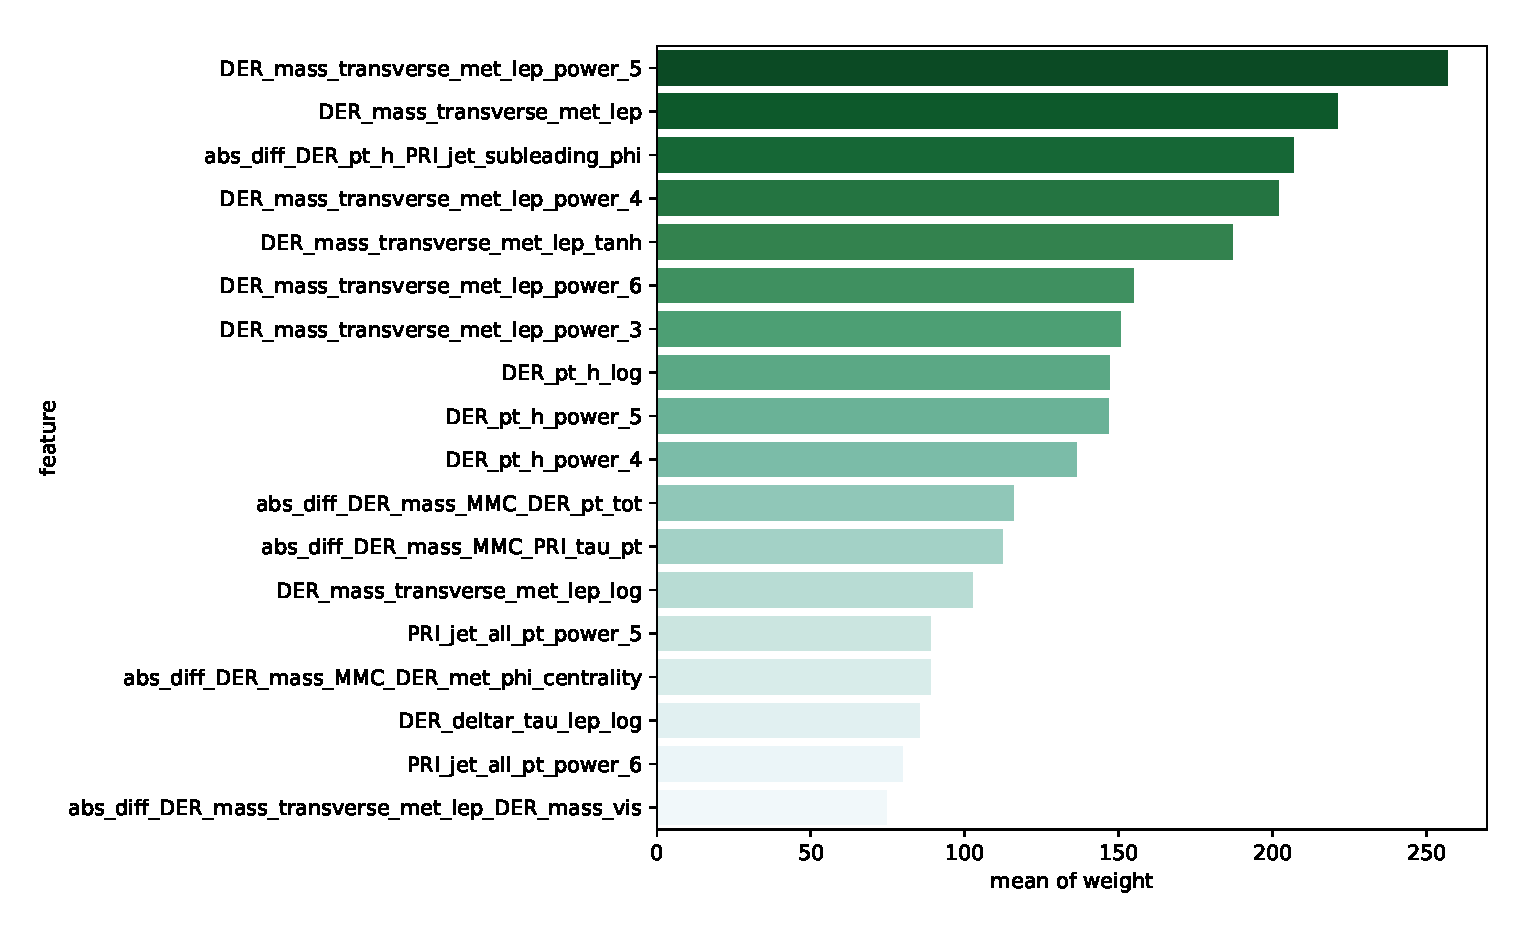
\includegraphics[width=\textwidth]{feature_importance.eps}
  \parbox{\textwidth}{
    \caption{Average absolute weight of the features which determine 50\% of the total weights. The given labels follow this naming schema: \texttt{\textless feature \textgreater\_\textless function\textgreater} for univariate and \texttt{\textless combinator \textgreater \_\textless feature a\textgreater\_\textless feature b\textgreater} for bivariate feature expansion.}}
  \label{feature_importance}
\end{figure}

%\addtolength{\textheight}{-12cm}   % This command serves to balance the column lengths
                                  % on the last page of the document manually. It shortens
                                  % the textheight of the last page by a suitable amount.
                                  % This command does not take effect until the next page
                                  % so it should come on the page before the last. Make
                                  % sure that you do not shorten the textheight too much.


\end{document}
